\section{Resultados e discussão}\label{sec:resultados}

Esta seção apresenta os resultados obtidos com a plataforma computacional descrita na Seção~\ref{sec:metodologia}, aplicada a dois casos de estudo hipotéticos de pontes de madeira roliça em estrada vicinal, doravante denominados Ponte~01 e Ponte~02. As duas configurações representam pontos distintos do espectro de demanda usualmente encontrado nesse tipo de obra: a Ponte~01 corresponde a um vão curto e a um tráfego leve ($L = 5{,}0$~m, trem tipo TB-240), representativo de acessos rurais de baixo volume de tráfego, enquanto a Ponte~02 corresponde a um vão maior e a um tráfego mais severo ($L = 8{,}0$~m, trem tipo TB-450), representativo de vias vicinais de maior importância regional. Optou-se por variar simultaneamente o vão e o trem tipo, em vez de isolar um único fator, de modo a aproximar os dois casos de estudo de situações de projeto reais, nas quais vãos maiores tendem a estar associados a vias de maior demanda de tráfego. Os parâmetros comuns às duas pontes, a configuração específica de cada caso e os intervalos das variáveis de projeto adotados na otimização são apresentados na Seção~\ref{sec:casos}.

Na sequência, apresenta-se brevemente a plataforma computacional desenvolvida (Seção~\ref{sec:plataforma}) e, em seguida, os resultados da otimização robusta multiobjetivo para os dois casos de estudo: as fronteiras eficientes (Seções~\ref{sec:ponte01} e~\ref{sec:ponte02}) e a análise comparativa entre os cenários (Seção~\ref{sec:comparacao}); o custo da robustez em função do nível de desvio adotado (Seção~\ref{sec:custo_robustez}) e sua validação por simulação de Monte Carlo independente (Seção~\ref{sec:validacao_mc}); a qualidade da fronteira aproximada, por meio do hipervolume e da convergência do algoritmo (Seção~\ref{sec:hipervolume}); e, por fim, a análise de sensibilidade global das variáveis de projeto (Seção~\ref{sec:sobol}) e a dispersão dessas variáveis ao longo da fronteira eficiente (Seção~\ref{sec:dispersao}).

\subsection{Plataforma computacional}\label{sec:plataforma}

Como principal produto de engenharia deste trabalho, foi desenvolvida uma plataforma computacional de acesso livre para o dimensionamento de pontes de madeira, capaz de realizar a verificação completa dos elementos estruturais em conformidade com as ABNT NBR 7190 \parencite{NBR7190-1:2022} e NBR 7188 \parencite{nbr7188}, disponível nos idiomas português e inglês \parencite{ReliaBridge2026}. A interface, ilustrada nas Figuras~\ref{fig:tela_inicial} e~\ref{fig:interface_dim}, é organizada em módulos que permitem a navegação sequencial entre as etapas de dimensionamento por otimização, projeto detalhado dos elementos e análise dos resultados. Ao final do processamento, a ferramenta disponibiliza para download a planilha de dados de entrada, os resultados do pré-dimensionamento e a imagem da fronteira de Pareto.

\begin{figure}[!ht]
    \centering
    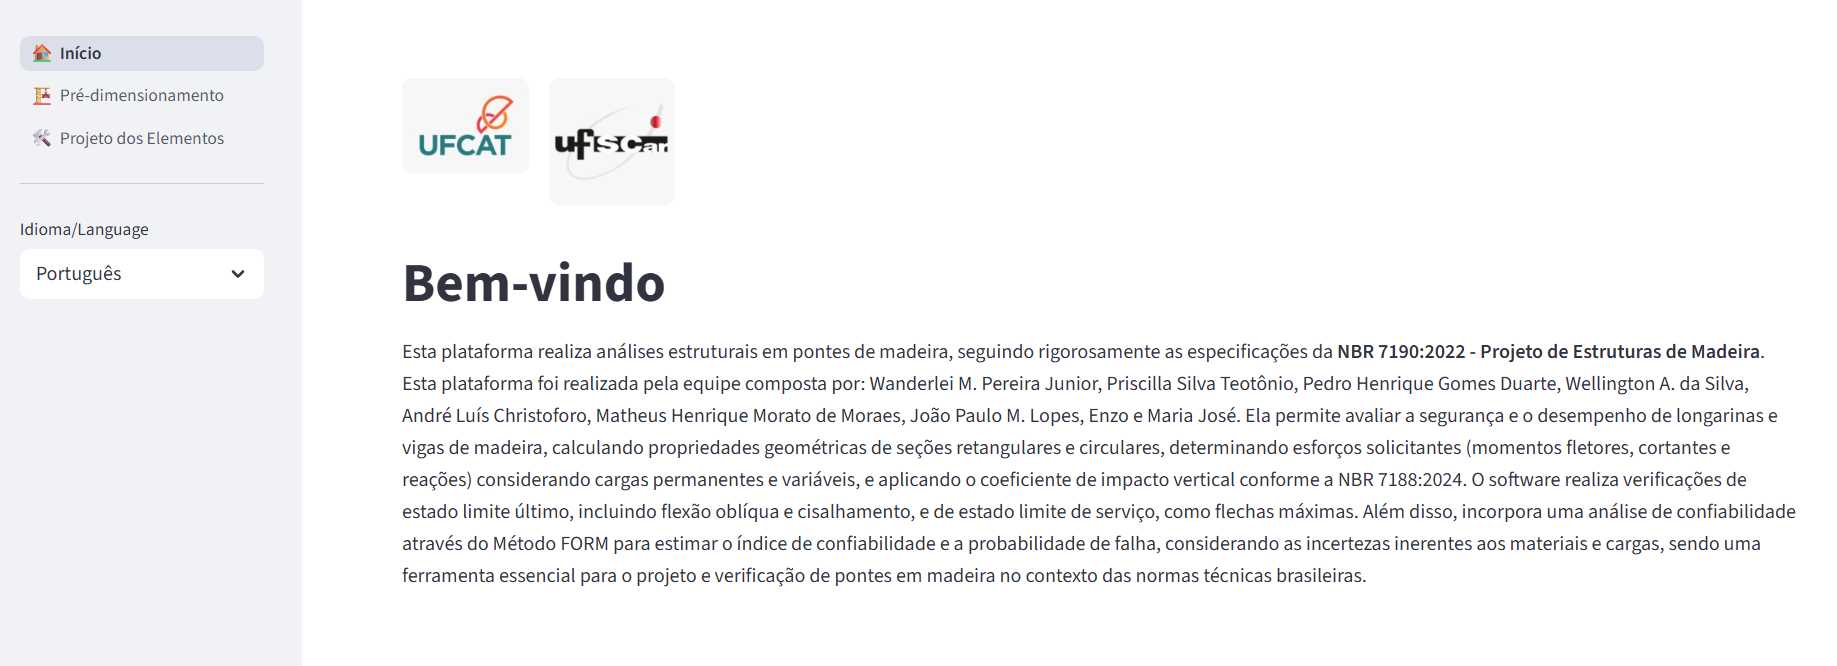
\includegraphics[width=0.85\textwidth]{figuras/interface_inicial.png}
    \caption{Tela inicial da plataforma computacional.}
    \label{fig:tela_inicial}
\end{figure}

\begin{figure}[!ht]
    \centering
    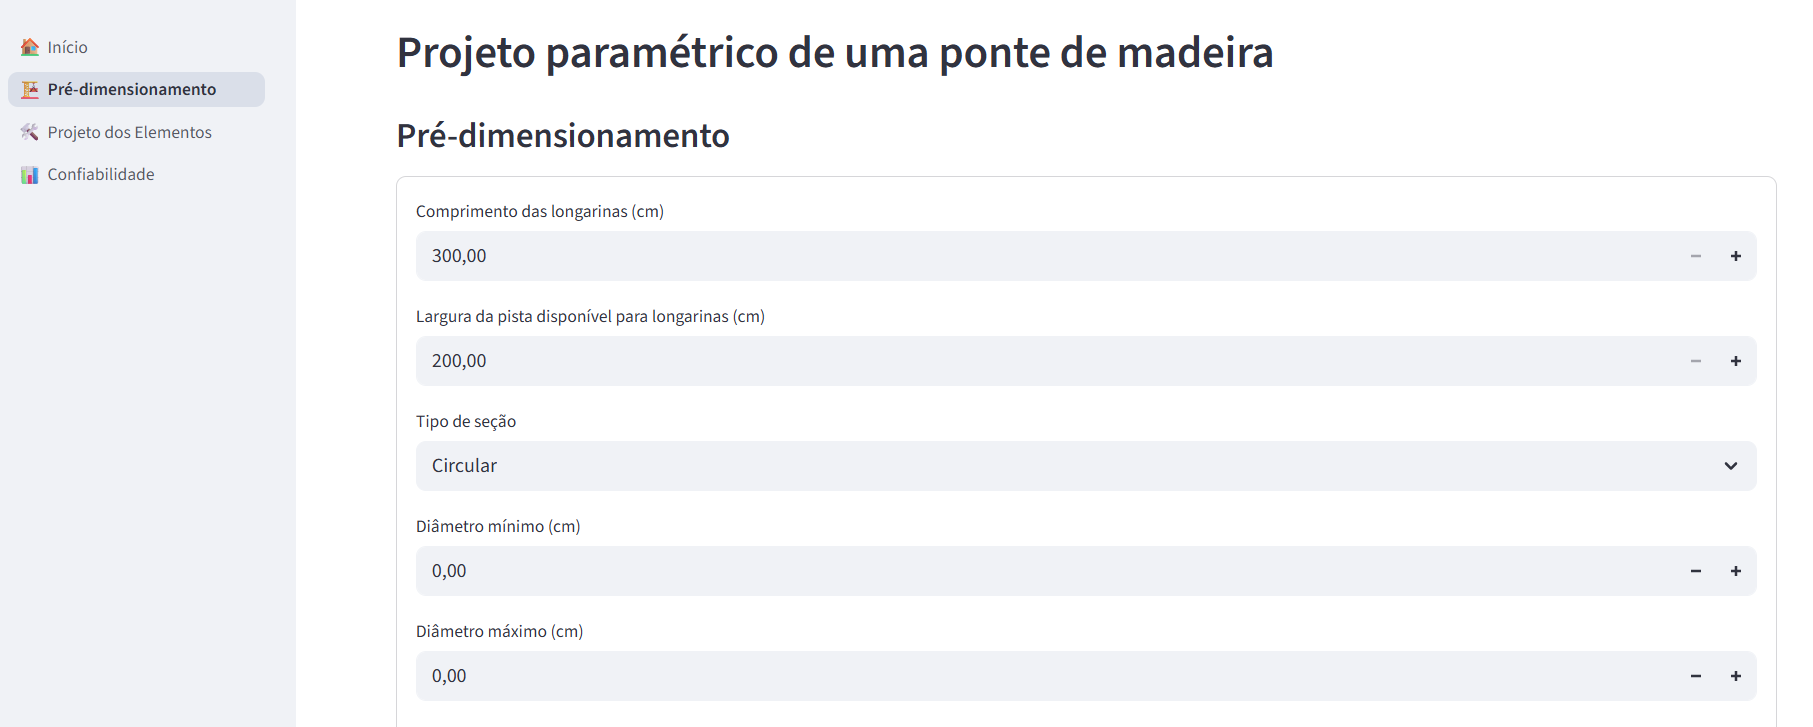
\includegraphics[width=0.9\textwidth]{figuras/interface_dimensionamento.png}
    \caption{Módulo de dimensionamento por otimização.}
    \label{fig:interface_dim}
\end{figure}

\subsection{Casos de estudo}\label{sec:casos}

Os parâmetros geométricos, mecânicos e os coeficientes normativos comuns às duas pontes são apresentados na Tabela~\ref{tab:parametros}; a configuração específica de cada caso -- vão e trem tipo -- na Tabela~\ref{tab:casos}; e os intervalos das variáveis de projeto adotados na otimização na Tabela~\ref{tab:intervalos}. A largura da pista, as propriedades mecânicas da madeira e os coeficientes normativos foram mantidos idênticos entre os dois casos, de modo que as diferenças observadas nos resultados decorram exclusivamente da combinação entre o vão e o trem tipo de cada cenário.

\begin{table}[!ht]
\caption{Parâmetros geométricos, mecânicos e coeficientes comuns às duas pontes.\label{tab:parametros}}
\begin{threeparttable}
\begin{tabular*}{\columnwidth}{@{\extracolsep\fill}lc@{\extracolsep\fill}}
\toprule
Parâmetro & Valor \\
\midrule
Largura da pista, $b_{w,\mathrm{pista}}$ (cm) & 900 \\
Carga permanente distribuída, $p_{gk}$ (kPa) & 1 \\
Distância entre eixos, $a$ (m) & 1{,}5 \\
Classe de carregamento & Permanente \\
Classe da madeira & Madeira natural \\
Classe de umidade & 1 \\
Coeficiente parcial das ações permanentes, $\gamma_g$ & 1{,}35 \\
Coeficiente parcial das ações variáveis, $\gamma_q$ & 1{,}50 \\
Coeficiente de minoração (tensões normais), $\gamma_{wf}$ & 1{,}40 \\
Coeficiente de minoração (cisalhamento), $\gamma_{wc}$ & 1{,}80 \\
Fator de combinação quase permanente, $\psi_2$ & 0{,}30 \\
Coeficiente de fluência, $\varphi$ & 0{,}60 \\
Densidade da madeira (kg/m\textsuperscript{3}) & 620 \\
Resistência característica à flexão, $f_{mk}$ (MPa) & 50 \\
Resistência característica ao cisalhamento, $f_{vk}$ (MPa) & 4 \\
Módulo de elasticidade à flexão, $E_{0,\mathrm{ef}}$ (GPa) & 14 \\
\bottomrule
\end{tabular*}
\end{threeparttable}
\end{table}

\begin{table}[!ht]
\caption{Configuração específica de cada caso de estudo.\label{tab:casos}}
\begin{threeparttable}
\begin{tabular*}{\columnwidth}{@{\extracolsep\fill}lcc@{\extracolsep\fill}}
\toprule
Parâmetro & Ponte 01 & Ponte 02 \\
\midrule
Vão teórico, $L$ (m) & 5{,}0 & 8{,}0 \\
Trem tipo (ABNT NBR 7188) & TB-240 & TB-450 \\
Carga concentrada por roda, $p_{rodak}$ (kN) & 40 & 75 \\
Carga variável distribuída, $p_{qk}$ (kPa) & 4 & 5 \\
\bottomrule
\end{tabular*}
\end{threeparttable}
\end{table}

\begin{table}[!ht]
\caption{Intervalos adotados para as variáveis de projeto.\label{tab:intervalos}}
\begin{threeparttable}
\begin{tabular*}{\columnwidth}{@{\extracolsep\fill}lcc@{\extracolsep\fill}}
\toprule
Variável & Valor mínimo (cm) & Valor máximo (cm) \\
\midrule
Diâmetro da longarina, $d$ & 30 & 150 \\
Largura da prancha do tabuleiro, $b_w$ & 5 & 60 \\
Altura da prancha do tabuleiro, $h$ & 5 & 60 \\
Espaçamento entre longarinas, $esp_{long}$ & 30 & 200 \\
Espaçamento entre peças do tabuleiro, $esp_{tab}$ & 5 & 60 \\
\bottomrule
\end{tabular*}
\end{threeparttable}
\end{table}

\subsection{Fronteira eficiente da Ponte 01 (TB-240, $L = 5$ m)}\label{sec:ponte01}

A otimização robusta multiobjetivo da Ponte~01 ($\rho = 5\%$) gerou um conjunto de soluções viáveis distribuídas ao longo da fronteira eficiente. A Tabela~\ref{tab:solucoes01} apresenta uma amostra representativa das soluções obtidas, com as respectivas funções objetivo e o maior valor entre as seis funções limite de restrição, confirmando o atendimento aos critérios normativos mesmo sob a avaliação robusta.

\begin{table}[!ht]
\caption{Soluções representativas da fronteira eficiente da Ponte 01 (TB-240).\label{tab:solucoes01}}
\begin{threeparttable}
\setlength{\tabcolsep}{3pt}
\begin{tabular*}{\textwidth}{@{\extracolsep{\fill}}ccccccc@{\extracolsep{\fill}}}
\toprule
$d$ (cm) & $b_w$ (cm) & $h$ (cm) & $esp_{long}$ (cm) & Volume (m\textsuperscript{3}) & $\delta_{\mathrm{tot}}/(L/250)$ & $g_{\max}$ \\
\midrule
\tofill{--} & \tofill{--} & \tofill{--} & \tofill{--} & \tofill{--} & \tofill{--} & \tofill{--} \\
\tofill{--} & \tofill{--} & \tofill{--} & \tofill{--} & \tofill{--} & \tofill{--} & \tofill{--} \\
\tofill{--} & \tofill{--} & \tofill{--} & \tofill{--} & \tofill{--} & \tofill{--} & \tofill{--} \\
\tofill{--} & \tofill{--} & \tofill{--} & \tofill{--} & \tofill{--} & \tofill{--} & \tofill{--} \\
\tofill{--} & \tofill{--} & \tofill{--} & \tofill{--} & \tofill{--} & \tofill{--} & \tofill{--} \\
\bottomrule
\end{tabular*}
\begin{tablenotes}
\footnotesize
\item \tofill{[A PREENCHER] Selecionar de 5 a 7 soluções da fronteira final, cobrindo do extremo de menor volume ao extremo de menor flecha adimensional. $g_{\max}$ é o maior valor entre $g_1$ a $g_6$ para a solução (deve ser $\leq 0$ para viabilidade).}
\end{tablenotes}
\end{threeparttable}
\end{table}

A fronteira eficiente é apresentada na Figura~\ref{fig:fronteira01}, relacionando o volume total de madeira com a utilizacao do limite de servico.

\begin{figure}[!ht]
    \centering
    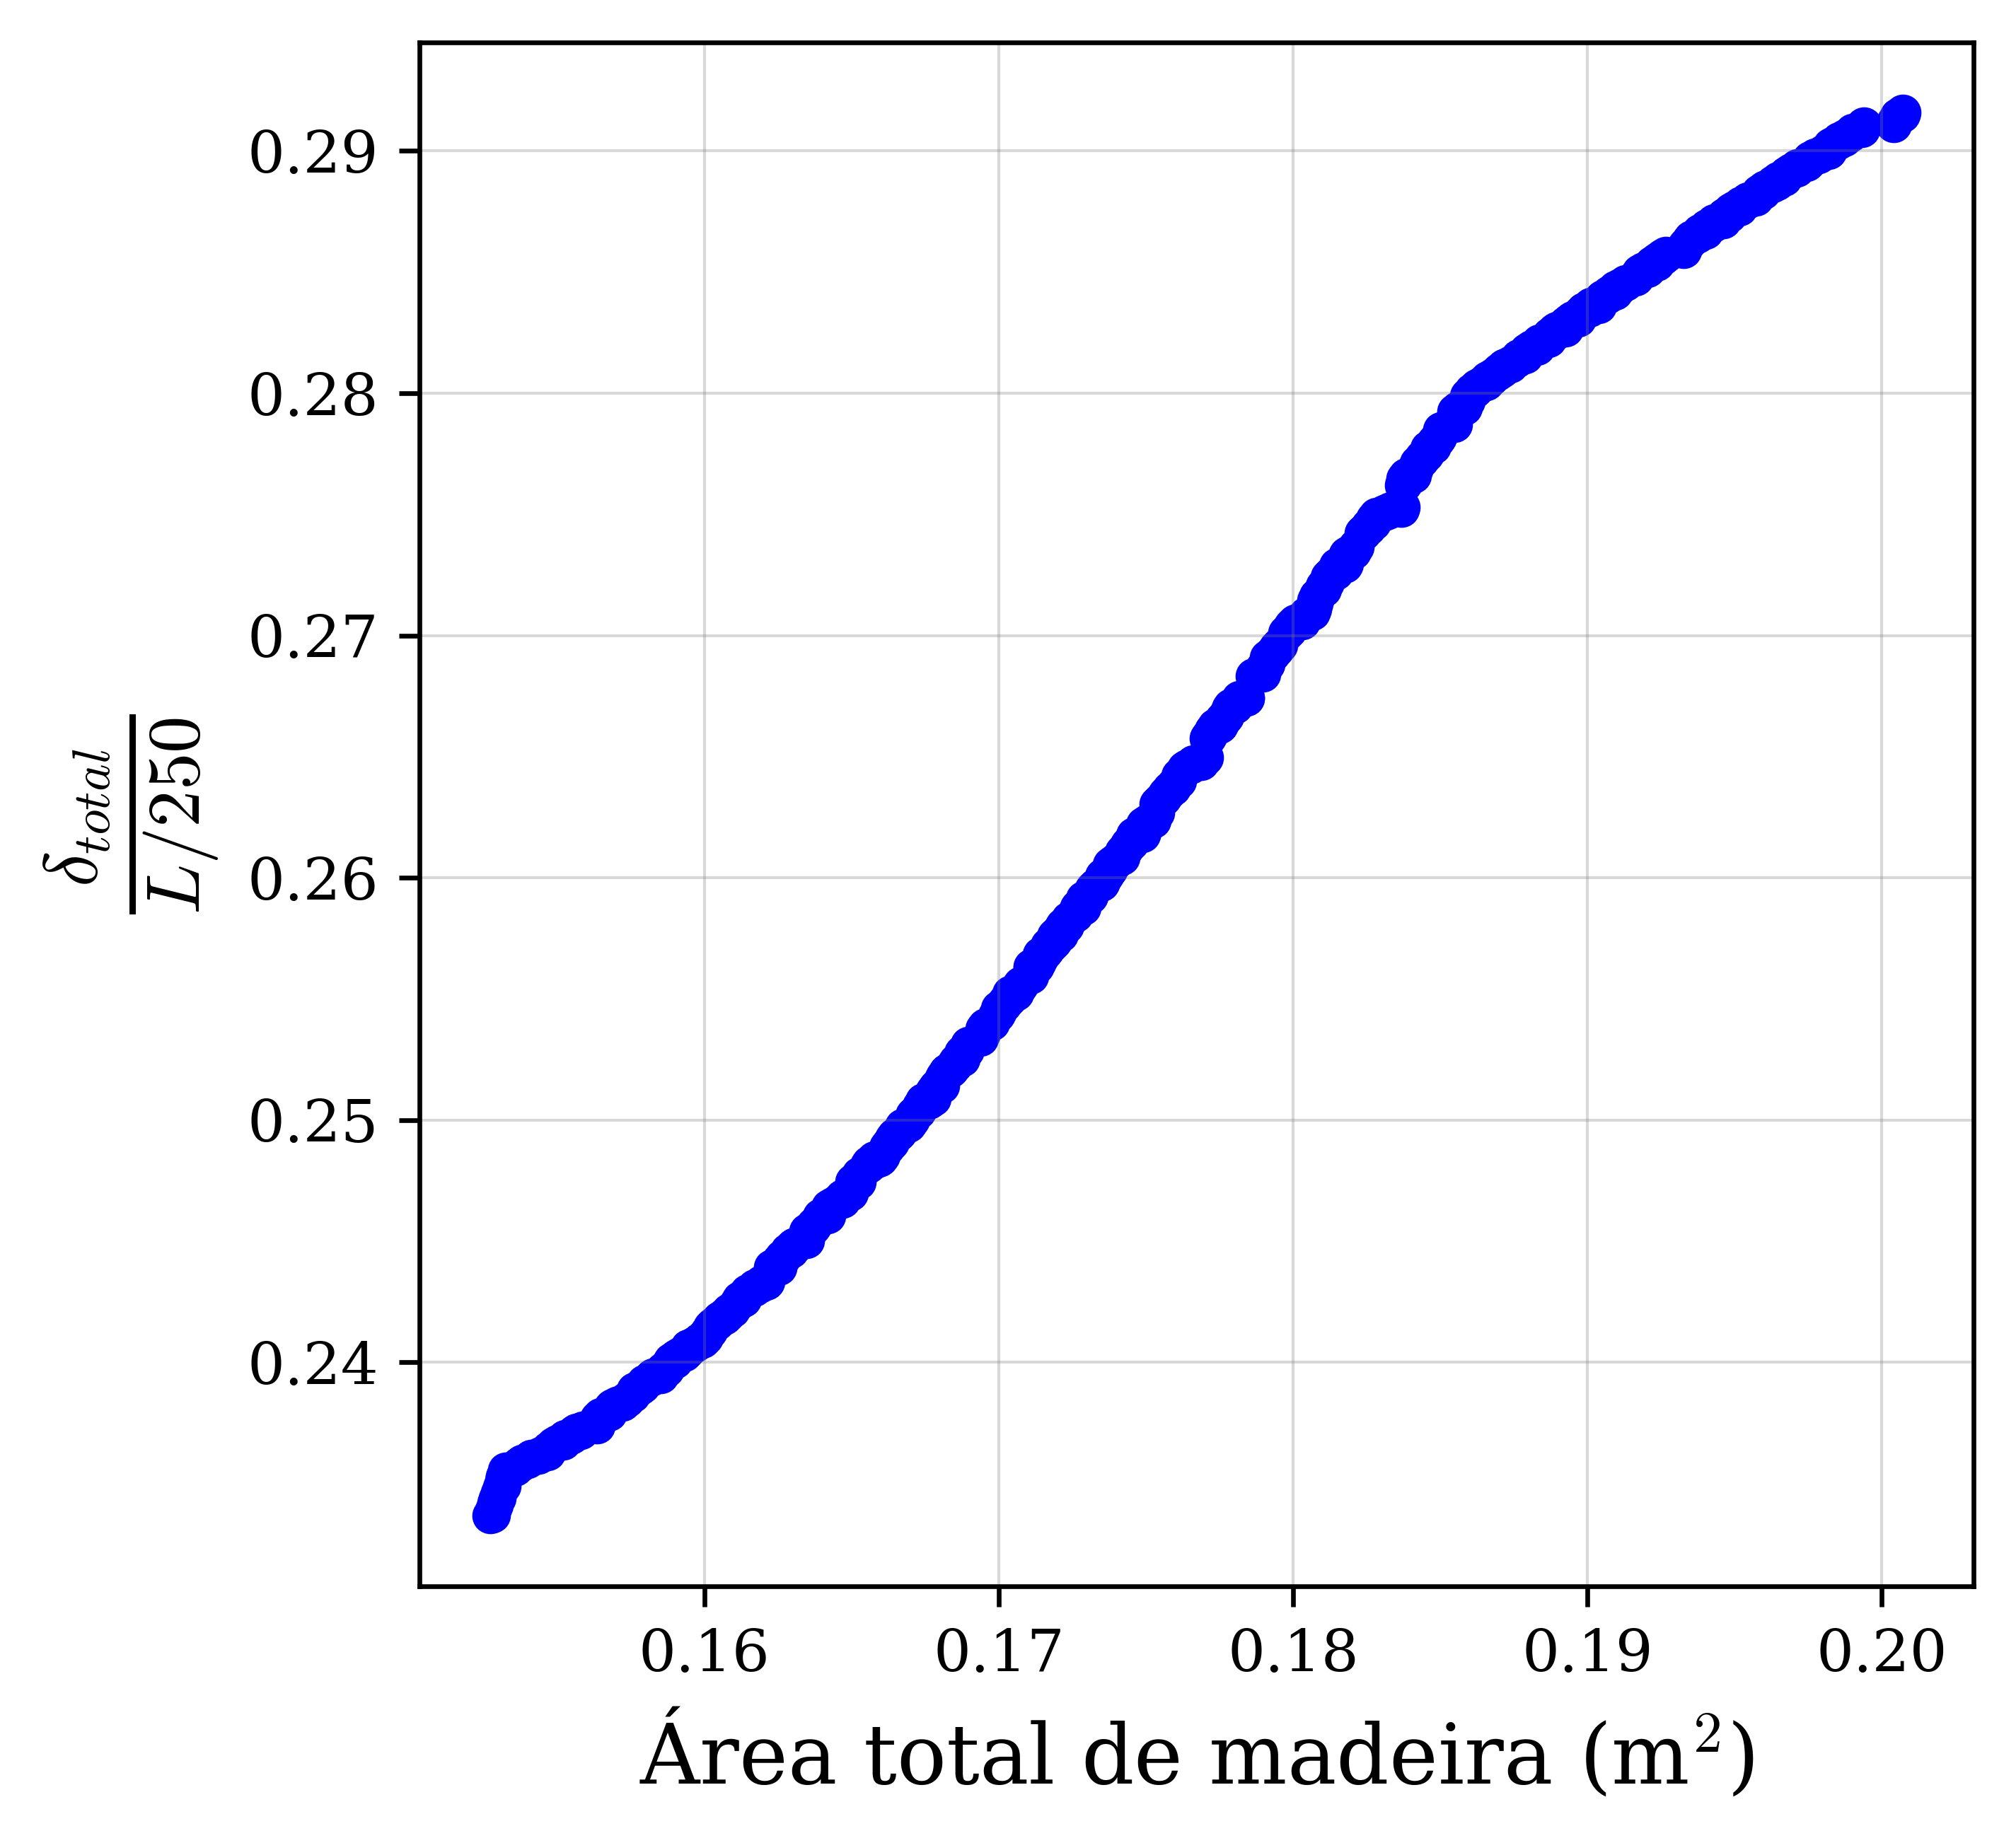
\includegraphics[width=0.55\textwidth]{figuras/z_fronteira_eficiente.png}
    \caption{Fronteira eficiente da Ponte 01 (TB-240). \tofill{[REGENERAR: figura atual foi produzida antes da correção da avaliação robusta; refazer com o algoritmo corrigido.]}}
    \label{fig:fronteira01}
\end{figure}

\tofill{[A PREENCHER] Descrever a tendência observada entre volume e utilizacao do limite de servico ao longo da fronteira (faixa de volume nos dois extremos da fronteira, em m\textsuperscript{3}).}

Para demonstrar a eficiência do processo de otimização, emprega-se o método de Monte Carlo para gerar um conjunto de soluções obtidas por amostragem aleatória, sem estratégia de otimização. A Figura~\ref{fig:mc01} compara as soluções aleatórias com a fronteira eficiente.

\begin{figure}[!ht]
    \centering
    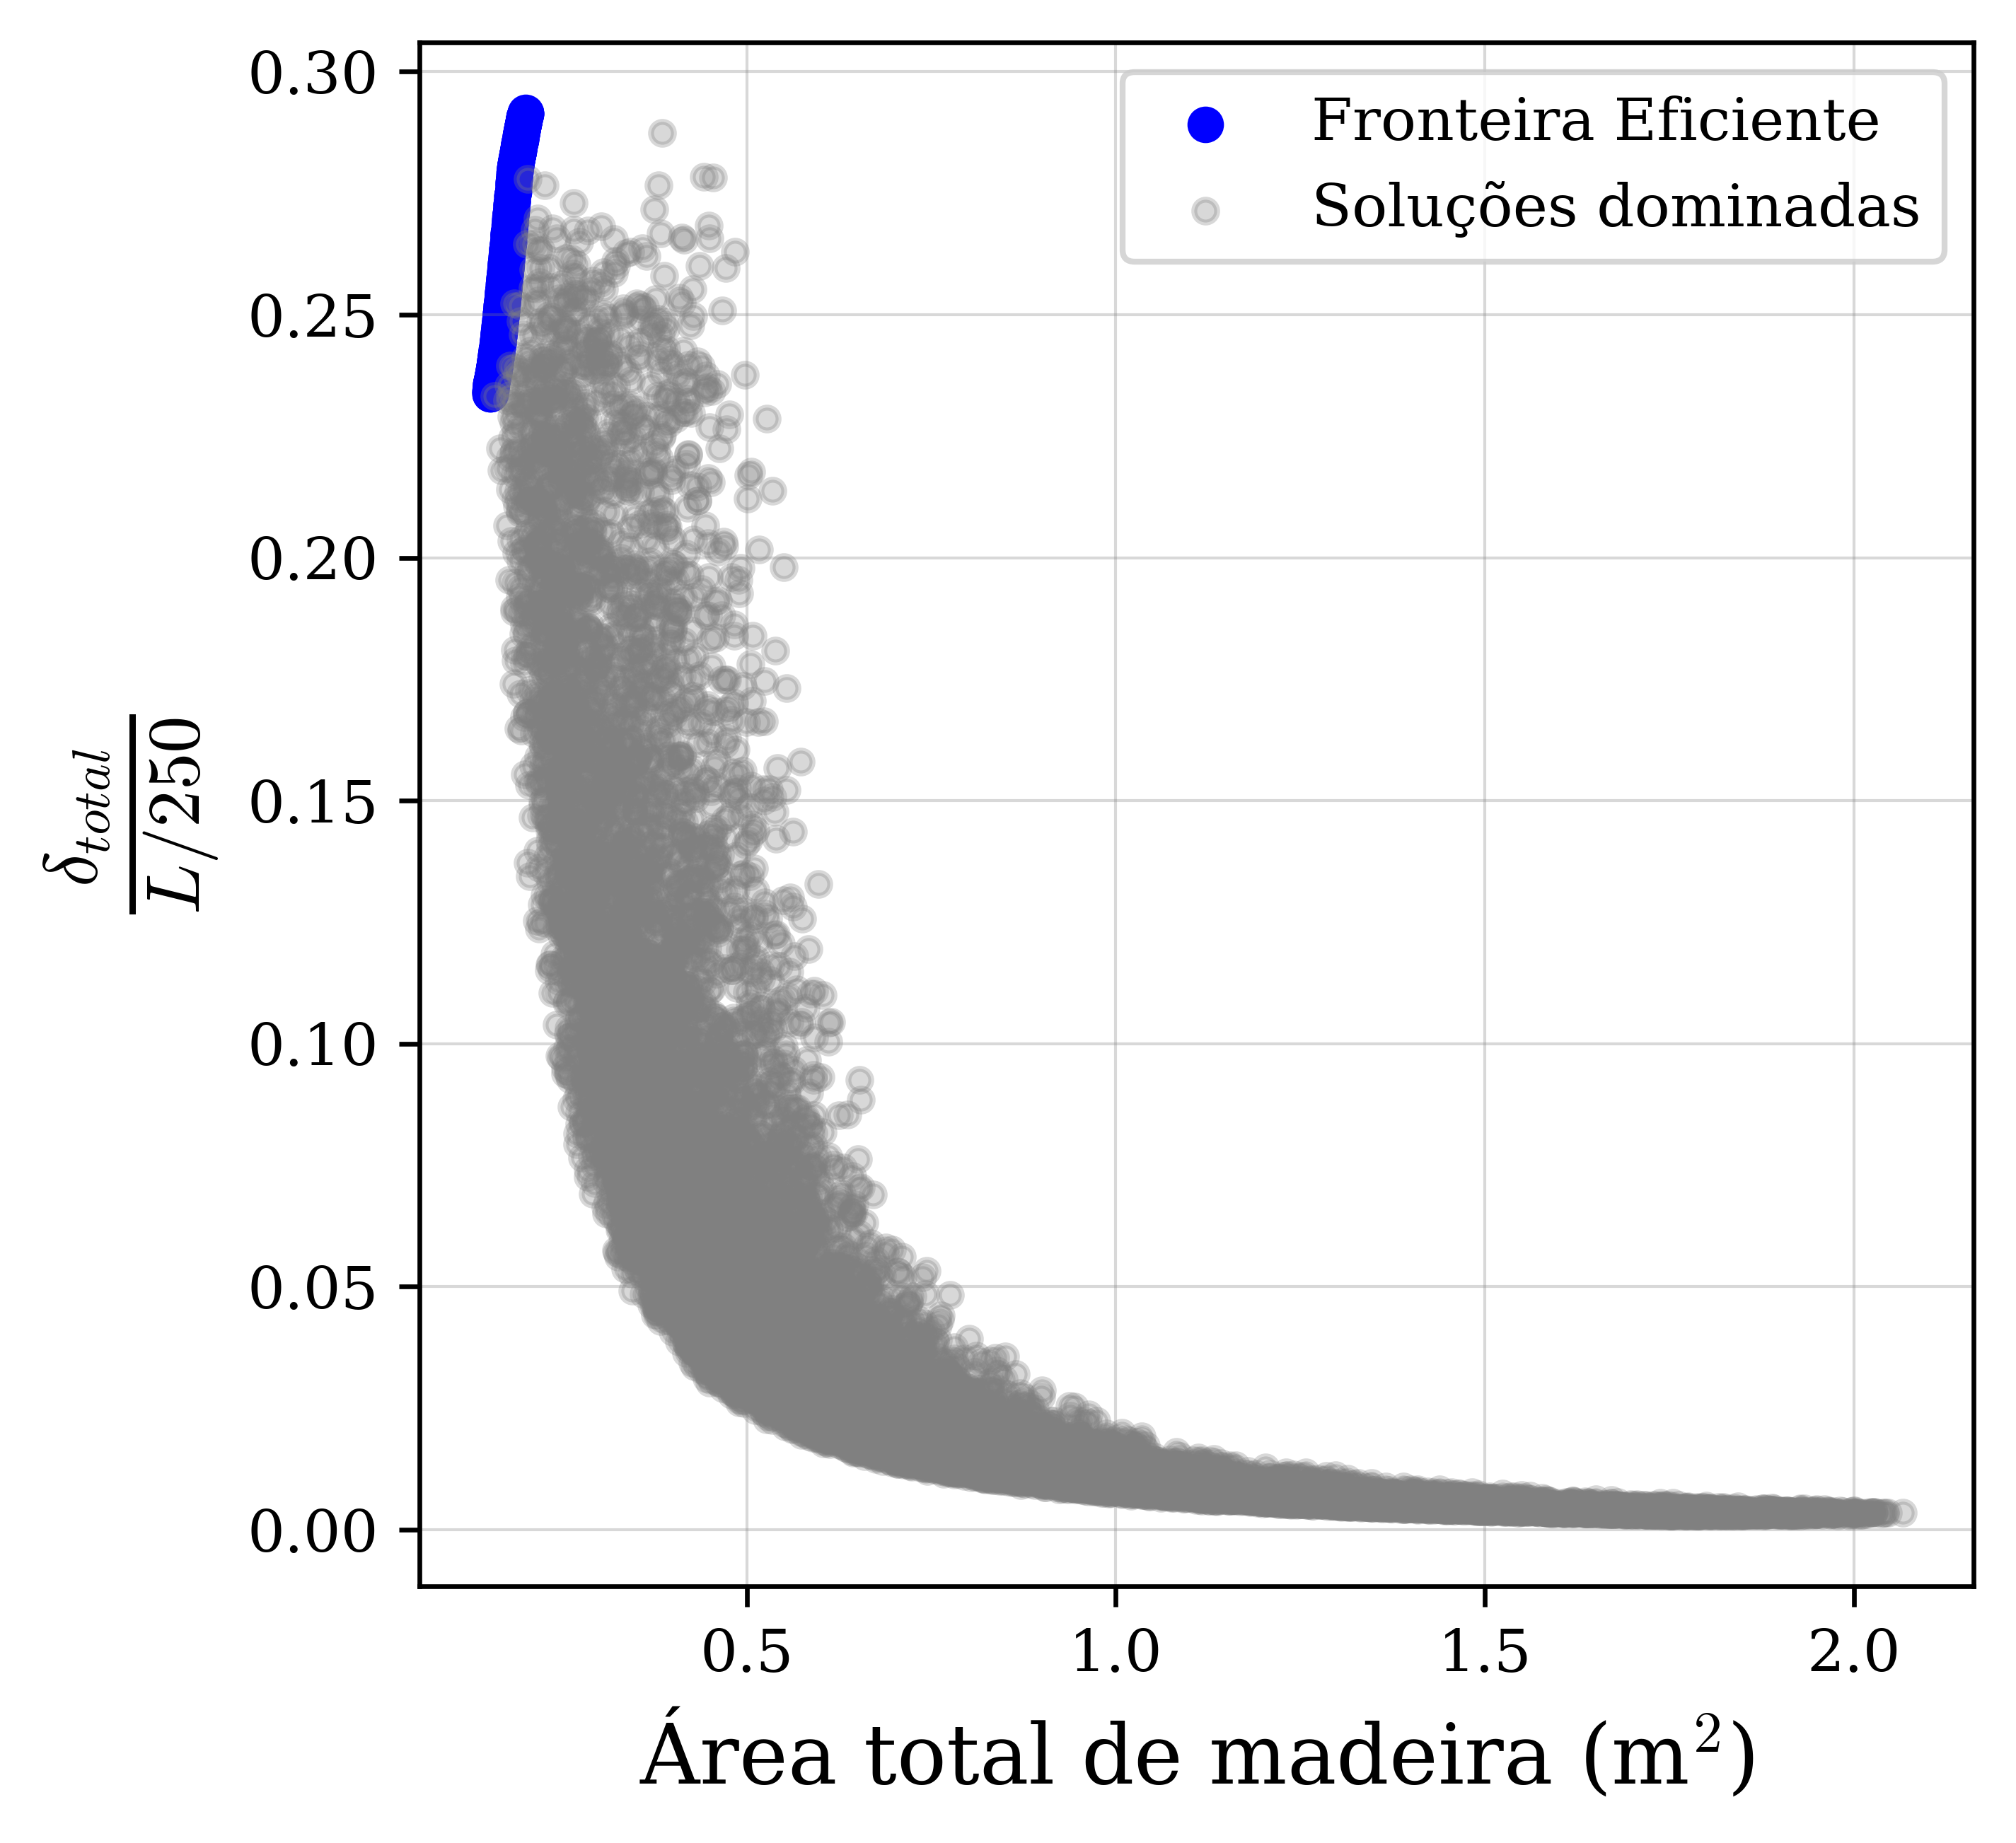
\includegraphics[width=0.55\textwidth]{figuras/z_fronteira_eficiente_vs_monte_carlo.png}
    \caption{Comparação entre a fronteira eficiente e as soluções por Monte Carlo (Ponte 01). \tofill{[REGENERAR]}}
    \label{fig:mc01}
\end{figure}

\tofill{[A PREENCHER] Discutir a comparação qualitativa: dispersão das soluções aleatórias, região de menor consumo de material ocupada pela fronteira de Pareto para cada nível de desempenho.}

Como complemento ao relatório de verificação do Apêndice~\ref{ap:relatorio}, a Figura~\ref{fig:utilizacao} apresenta o grau de utilização (razão entre solicitação e resistência, ou entre deslocamento e limite admissível) de cada verificação normativa, para a solução selecionada no Apêndice~\ref{ap:demonstracao}.

\begin{figure}[!ht]
    \centering
    \includegraphics[width=0.75\textwidth]{figuras/utilizacao_ponte01.png}
    \caption{Grau de utilização de cada verificação normativa, para a solução selecionada da fronteira robusta da Ponte 01.}
    \label{fig:utilizacao}
\end{figure}

\begin{fillblock}
\noindent\textbf{[A PREENCHER]} Gerar a Figura~\ref{fig:utilizacao} como um gráfico de barras horizontais, uma barra por verificação ($g_1$ a $g_4$, flexão e cisalhamento da longarina, flecha e flexão do tabuleiro), com o grau de utilização em \% no eixo horizontal (100\% = limite normativo). Discutir qual verificação está mais próxima do limite (mais restritiva) e qual apresenta maior folga.
\end{fillblock}

\subsection{Fronteira eficiente da Ponte 02 (TB-450, $L = 8$ m)}\label{sec:ponte02}

O processo foi repetido para a Ponte~02, com vão de 8{,}0~m e trem tipo TB-450. Os resultados são ilustrados nas Figuras~\ref{fig:fronteira02} e~\ref{fig:mc02}.

\begin{figure}[!ht]
    \centering
    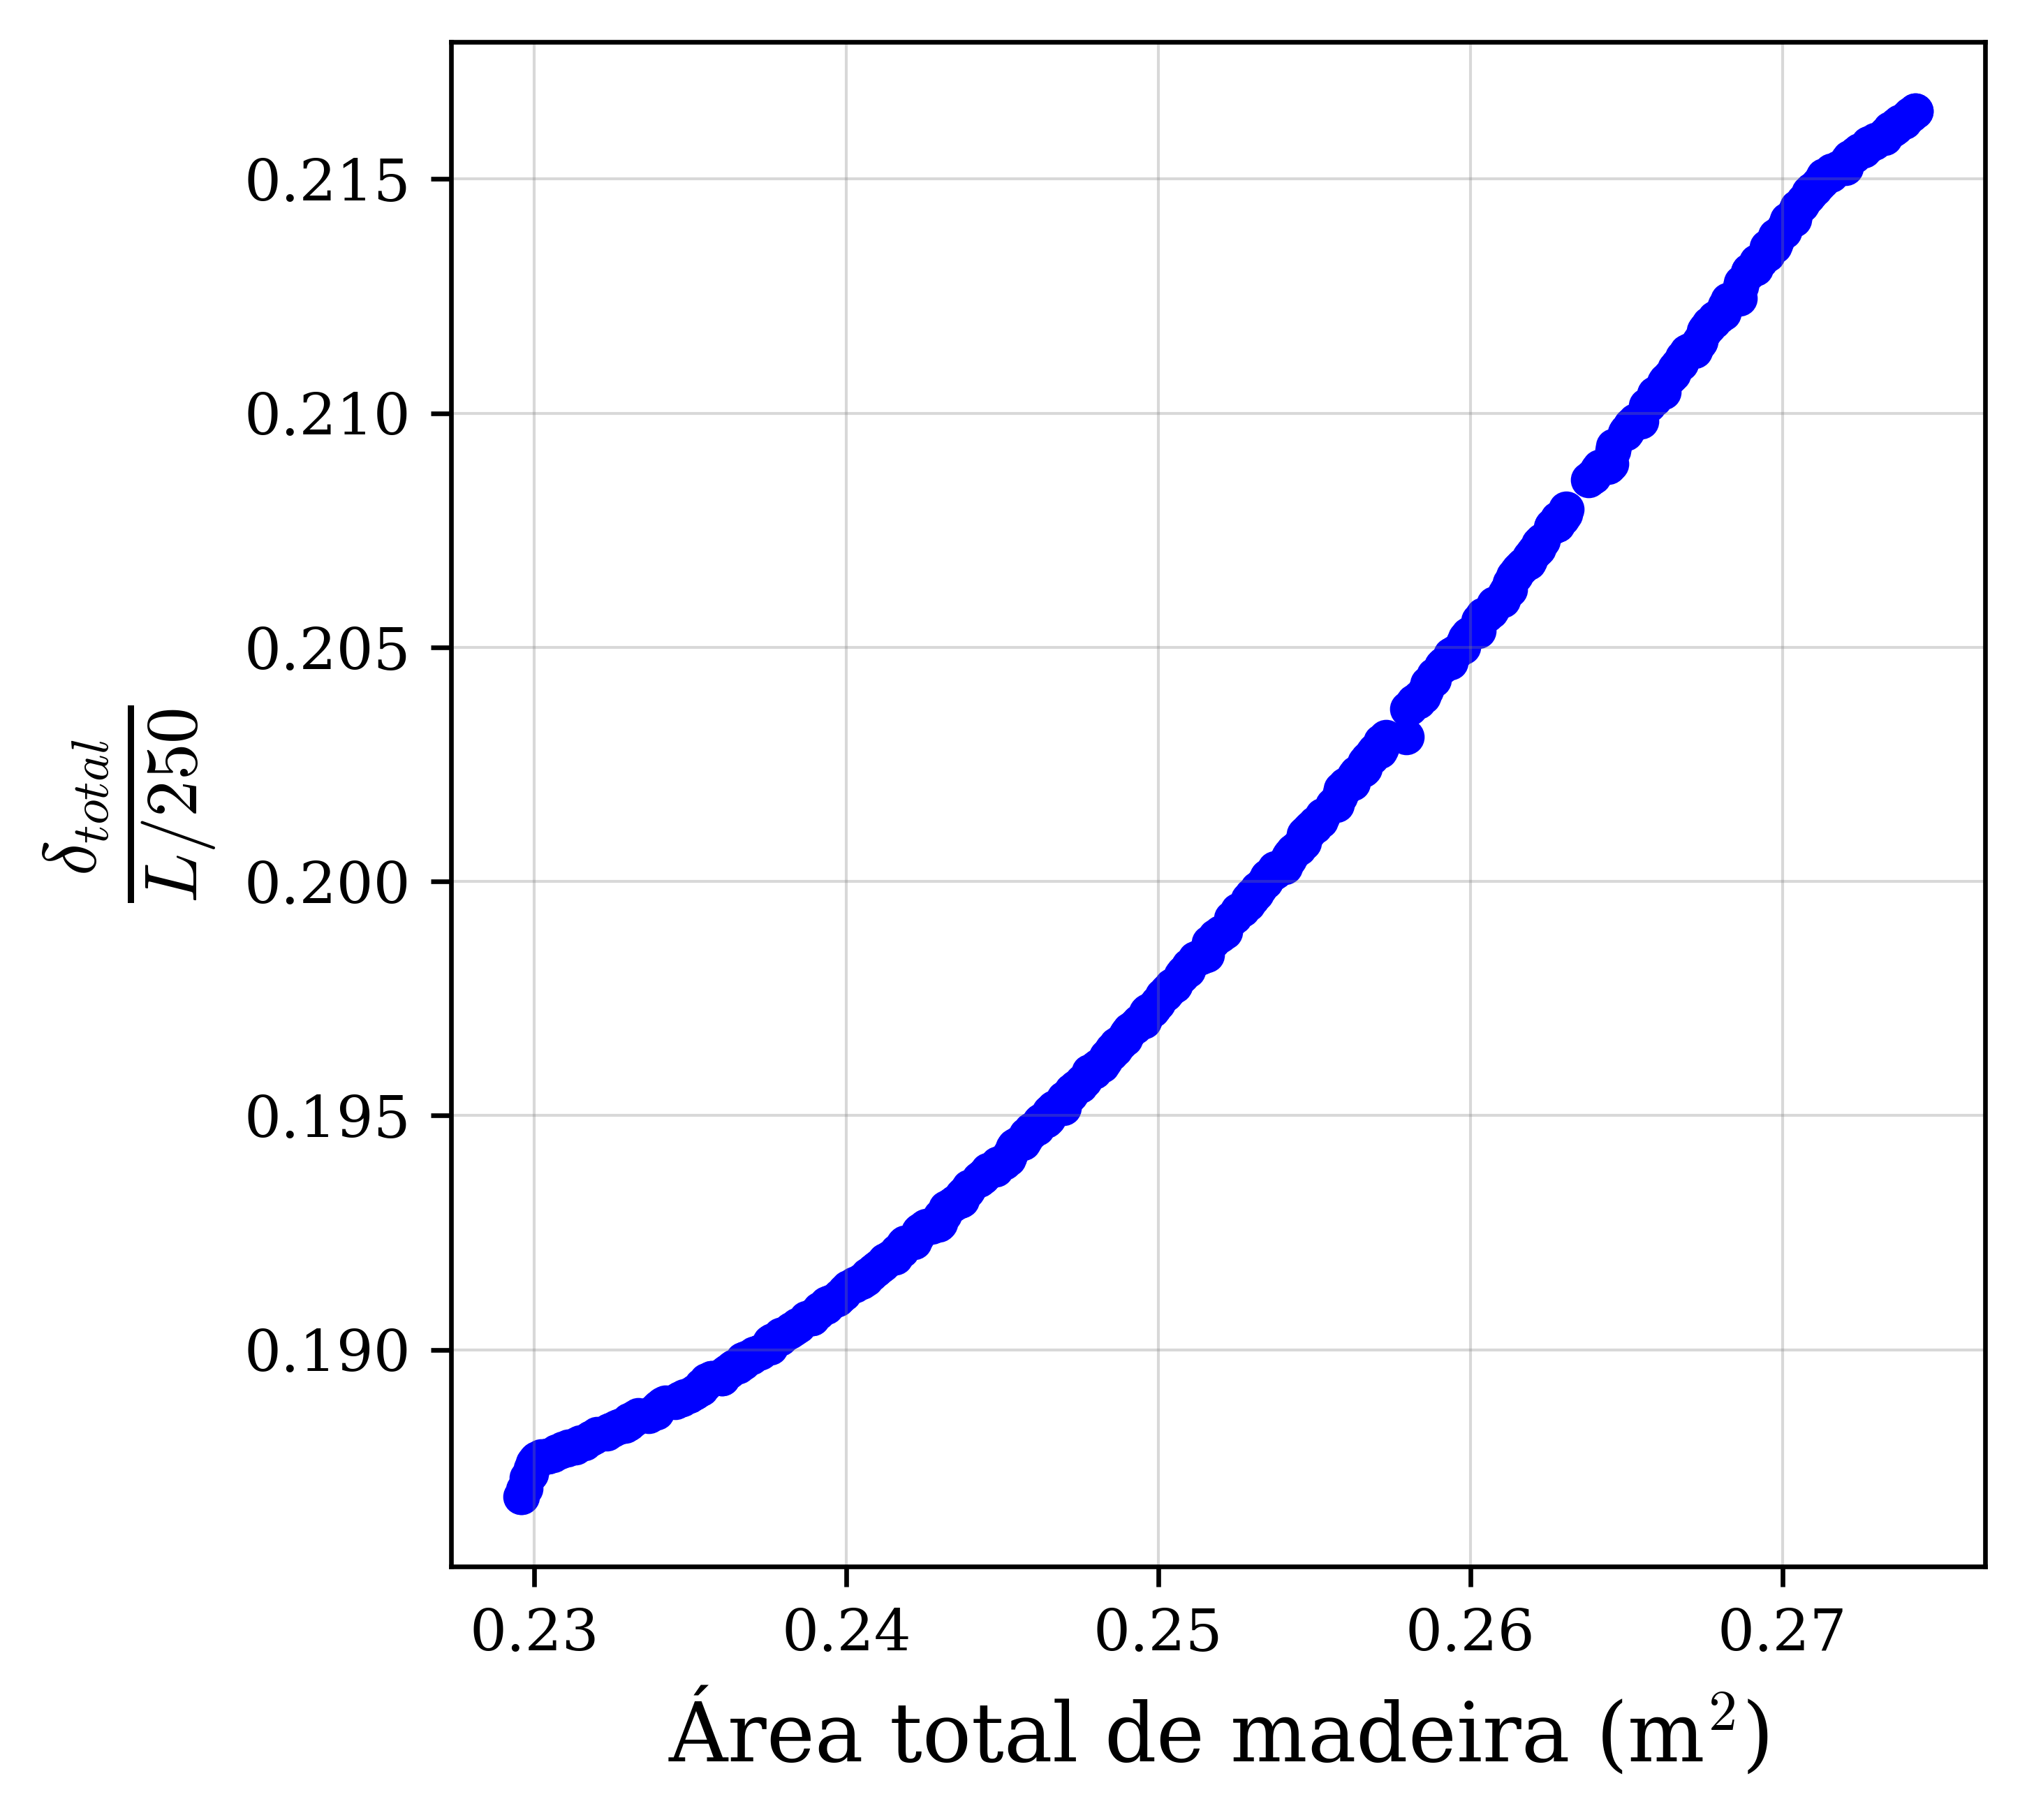
\includegraphics[width=0.55\textwidth]{figuras/z_fronteira_eficiente_viga2.png}
    \caption{Fronteira eficiente da Ponte 02 (TB-450). \tofill{[REGENERAR: figura atual corresponde à configuração antiga (L = 5 m); refazer para L = 8 m.]}}
    \label{fig:fronteira02}
\end{figure}

\begin{figure}[!ht]
    \centering
    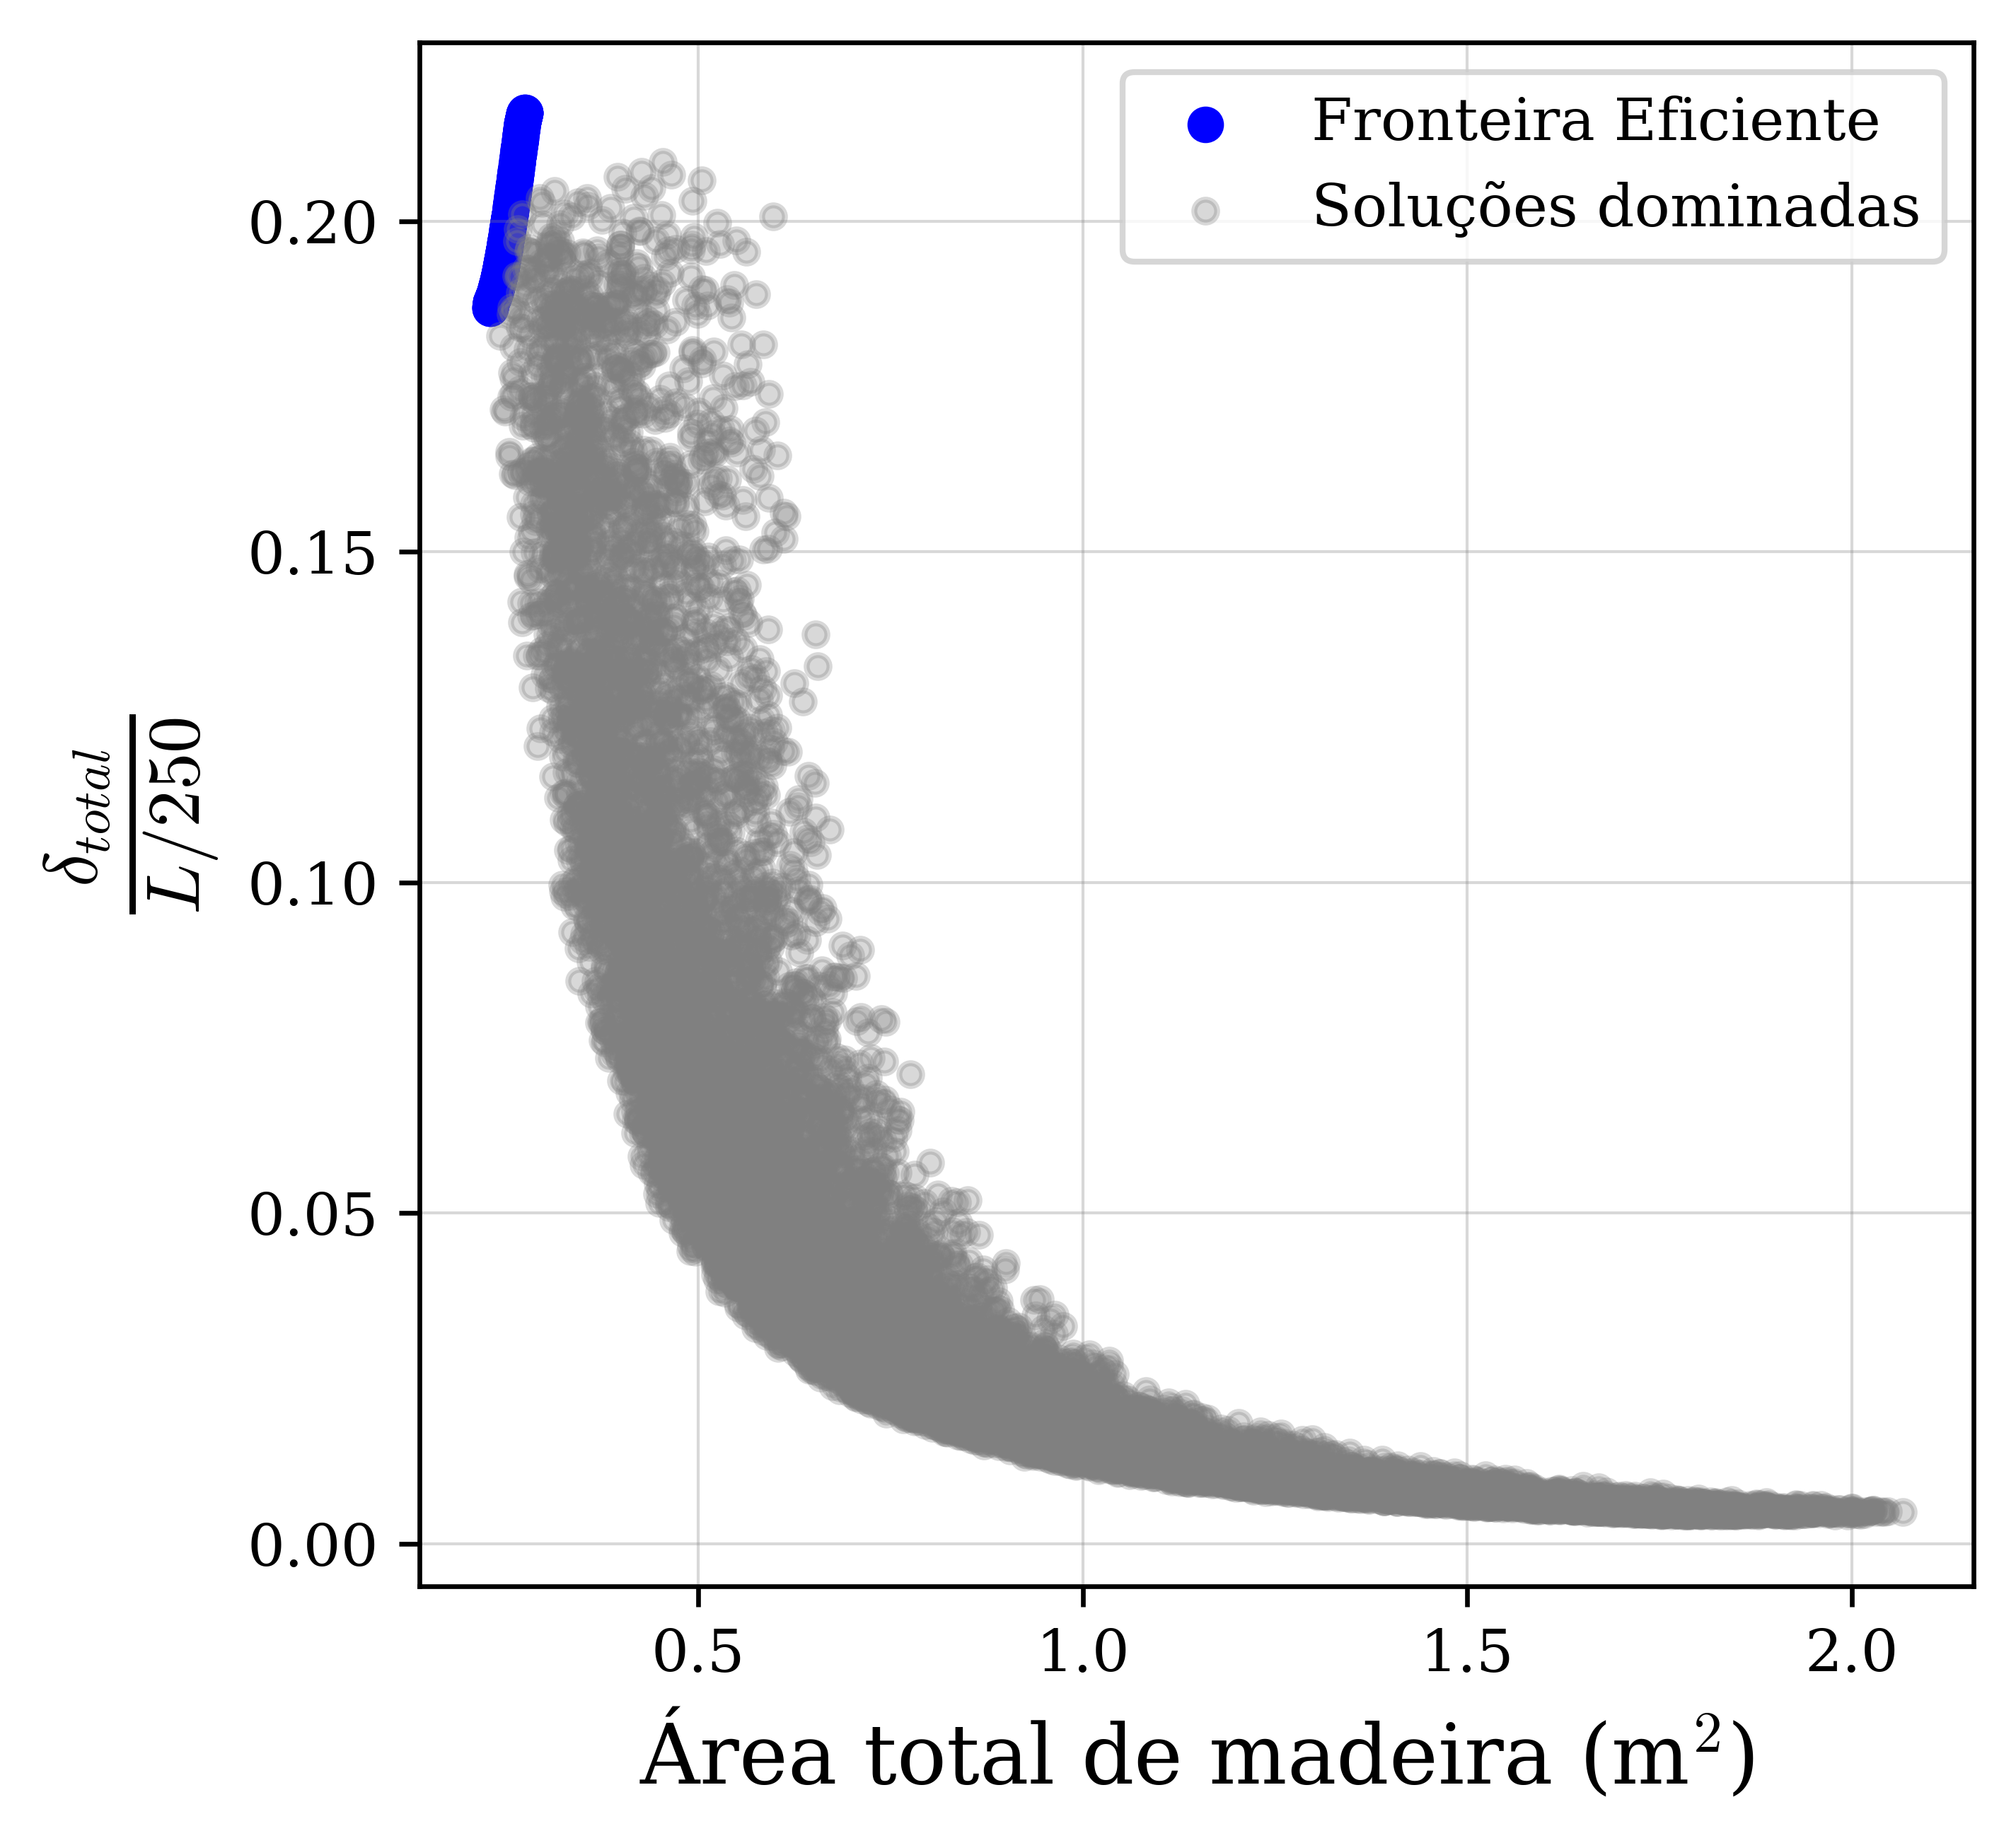
\includegraphics[width=0.55\textwidth]{figuras/z_fronteira_eficiente_vs_monte_carlo_viga2.png}
    \caption{Comparação entre a fronteira eficiente e as soluções por Monte Carlo (Ponte 02). \tofill{[REGENERAR]}}
    \label{fig:mc02}
\end{figure}

\tofill{[A PREENCHER] Descrever se o comportamento qualitativo (tendência volume x utilizacao, superioridade frente ao Monte Carlo) se mantém em relação à Ponte 01, e destacar diferenças relevantes decorrentes do vão maior e do trem tipo mais severo.}

\subsection{Análise comparativa entre os cenários}\label{sec:comparacao}

A Tabela~\ref{tab:comparacao} resume os volumes totais de madeira obtidos para cada cenário, incluindo valores mínimos, máximos e médios ao longo da fronteira eficiente, bem como o acréscimo percentual da Ponte~02 em relação à Ponte~01.

\begin{table}[!ht]
\caption{Comparação dos volumes totais de madeira para os dois casos de estudo.\label{tab:comparacao}}
\begin{threeparttable}
\begin{tabular*}{\columnwidth}{@{\extracolsep\fill}lccc@{\extracolsep\fill}}
\toprule
Cenário & Mínimo (m\textsuperscript{2}) & Máximo (m\textsuperscript{2}) & Média (m\textsuperscript{2}) \\
\midrule
Ponte 01 ($L=5$ m, TB-240) & \tofill{--} & \tofill{--} & \tofill{--} \\
Ponte 02 ($L=8$ m, TB-450) & \tofill{--} & \tofill{--} & \tofill{--} \\
\midrule
Acréscimo (\%) & \tofill{--} & \tofill{--} & \tofill{--} \\
\bottomrule
\end{tabular*}
\end{threeparttable}
\end{table}

\begin{fillblock}
\noindent\textbf{[A PREENCHER]} Como o vão e o trem tipo variam simultaneamente entre os dois casos, o acréscimo de volume reportado na Tabela~\ref{tab:comparacao} reflete o efeito combinado dos dois fatores, e não apenas do carregamento móvel (diferentemente da versão anterior deste trabalho, em que a geometria era mantida fixa). Discutir separadamente, de forma qualitativa, a contribuição esperada de cada fator: o aumento do vão eleva o momento fletor com $L^2$ (ação permanente) e aproximadamente de forma linear a quadrática (ação variável, conforme a extensão do trem tipo em relação ao vão -- Equações~\eqref{eq:mqk30} e~\eqref{eq:mqk45}), enquanto o trem tipo mais severo eleva diretamente a carga por roda e a carga de multidão. Relacionar o acréscimo total observado com essas duas contribuições.
\end{fillblock}

\subsection{Custo da robustez}\label{sec:custo_robustez}

A otimização determinística tende a posicionar as soluções ótimas exatamente sobre a fronteira das restrições ativas, tornando-as sensíveis a pequenas variações nas variáveis de projeto. Em pontes de madeira roliça, essa sensibilidade é agravada pela variabilidade natural do diâmetro das peças e pelas tolerâncias de fabricação e montagem. A incorporação da robustez desloca a fronteira eficiente para o interior do domínio viável: enquanto a otimização determinística tende a produzir soluções com função limite de flexão da longarina exatamente nula ($g_1 \approx 0$), a otimização robusta penaliza essas soluções, pois sob perturbação de $\pm\rho$ parte das realizações resultaria em violação.

Para quantificar esse efeito, a Ponte~01 foi reotimizada para quatro níveis de desvio, $\rho \in \{0\%,\ 2{,}5\%,\ 5\%,\ 10\%\}$, mantendo os demais parâmetros do algoritmo inalterados (Tabela~\ref{tab:nsga2}). O caso $\rho = 0\%$ corresponde à otimização determinística ($N_c = 1$), usada como referência.

\begin{figure}[!ht]
    \centering
    \includegraphics[width=0.7\textwidth]{figuras/custo_robustez_ponte01.png}
    \caption{Fronteiras eficientes da Ponte 01 para $\rho = 0\%,\ 2{,}5\%,\ 5\%$ e $10\%$.}
    \label{fig:custo_robustez}
\end{figure}

\begin{table}[!ht]
\caption{Acréscimo percentual de volume em relação ao caso determinístico ($\rho = 0\%$), para três níveis pareados de flecha adimensional.\label{tab:custo_robustez}}
\begin{threeparttable}
\begin{tabular*}{\columnwidth}{@{\extracolsep\fill}lccccccc@{\extracolsep\fill}}
\toprule
$\delta_{\mathrm{tot}}/(L/250)$ & $V(0\%)$ & $V(2{,}5\%)$ & $\Delta$ & $V(5\%)$ & $\Delta$ & $V(10\%)$ & $\Delta$ \\
\midrule
\tofill{--} & \tofill{--} & \tofill{--} & \tofill{--\%} & \tofill{--} & \tofill{--\%} & \tofill{--} & \tofill{--\%} \\
\tofill{--} & \tofill{--} & \tofill{--} & \tofill{--\%} & \tofill{--} & \tofill{--\%} & \tofill{--} & \tofill{--\%} \\
\tofill{--} & \tofill{--} & \tofill{--} & \tofill{--\%} & \tofill{--} & \tofill{--\%} & \tofill{--} & \tofill{--\%} \\
\bottomrule
\end{tabular*}
\begin{tablenotes}
\footnotesize
\item Volume em m\textsuperscript{3}; $\Delta$ = acréscimo percentual em relação a $V(0\%)$, para o mesmo nível de $\delta_{\mathrm{tot}}/(L/250)$.
\end{tablenotes}
\end{threeparttable}
\end{table}

\begin{fillblock}
\noindent\textbf{[A PREENCHER]} Discutir a Figura~\ref{fig:custo_robustez} e a Tabela~\ref{tab:custo_robustez}: verificar se o deslocamento da fronteira para o interior do domínio viável é monotônico em $\rho$; relatar o tempo de processamento de cada uma das quatro execuções (revisor de otimização costuma perguntar); e concluir explicitamente quanto material a mais custa cada nível adicional de tolerância a desvios dimensionais -- este é o resultado central de originalidade do trabalho.
\end{fillblock}

\subsection{Validação por simulação de Monte Carlo independente}\label{sec:validacao_mc}

Para verificar empiricamente o ganho de robustez, seleciona-se uma solução da fronteira determinística ($\rho = 0\%$) e uma solução de volume equivalente da fronteira robusta ($\rho = 5\%$), ambas da Ponte~01 (Seção~\ref{sec:custo_robustez}). Para cada uma, geram-se $10^4$ realizações perturbadas, $\tilde{\mathbf{x}} = \mathbf{x}\,(1+\rho\,\boldsymbol{\xi})$, com $\boldsymbol{\xi}\sim\mathcal{U}(-1,1)$ e semente aleatória distinta da utilizada na otimização, e avalia-se o percentual de realizações que violam cada uma das seis restrições do modelo, bem como a probabilidade de violação do sistema (violação de ao menos uma restrição).

\begin{table}[!ht]
\caption{Percentual de realizações perturbadas que violam cada restrição ($10^4$ amostras, $\rho = 5\%$).\label{tab:validacao_mc}}
\begin{threeparttable}
\begin{tabular*}{\columnwidth}{@{\extracolsep\fill}lcc@{\extracolsep\fill}}
\toprule
Restrição & Solução determinística & Solução robusta \\
\midrule
$g_1$ -- flexão longarina & \tofill{--\%} & \tofill{--\%} \\
$g_2$ -- cisalhamento longarina & \tofill{--\%} & \tofill{--\%} \\
$g_3$ -- flecha longarina & \tofill{--\%} & \tofill{--\%} \\
$g_4$ -- flexão tabuleiro & \tofill{--\%} & \tofill{--\%} \\
$g_5$ -- espaçamento longarinas & \tofill{--\%} & \tofill{--\%} \\
$g_6$ -- espaçamento tabuleiro & \tofill{--\%} & \tofill{--\%} \\
\midrule
Sistema (qualquer uma) & \tofill{--\%} & \tofill{--\%} \\
\bottomrule
\end{tabular*}
\end{threeparttable}
\end{table}

\begin{fillblock}
\noindent\textbf{[A PREENCHER]} Discutir a Tabela~\ref{tab:validacao_mc}, com atenção a dois pontos: (i) como a formulação adotada agrega as restrições pela média (Seção~\ref{sec:robustez}), é esperado que a solução robusta ainda viole a restrição mais ativa em uma fração não desprezível das realizações -- reportar esse valor sem maquiar o resultado é mais convincente do que escondê-lo; (ii) a linha ``Sistema'' é a comparação mais relevante para o projetista, pois representa a probabilidade de falha considerando todos os modos de falha simultaneamente.
\end{fillblock}

\subsection{Qualidade da fronteira: hipervolume e convergência}\label{sec:hipervolume}

A qualidade de uma fronteira aproximada é avaliada, de forma independente da inspeção visual, pelo indicador de hipervolume (HV), que mede a fração do espaço objetivo dominada pela fronteira em relação a um ponto de referência $\mathbf{r}$, conforme a Equação~\eqref{eq:hv} \parencite{blank2020}.

\begin{equation}
HV(\mathcal{F}_1, \mathbf{r}) = \mathrm{Vol}\left(\bigcup_{\mathbf{x} \in \mathcal{F}_1} \left[f_1(\mathbf{x}), r_1\right] \times \left[f_2(\mathbf{x}), r_2\right]\right)
\label{eq:hv}
\end{equation}

A Figura~\ref{fig:convergencia_hv} apresenta a evolução do hipervolume em função do número de gerações, para as Pontes~01 e~02 ($\rho = 5\%$), justificando a escolha de $N_{gen} = 300$ (Tabela~\ref{tab:nsga2}).

\begin{figure}[!ht]
    \centering
    
\includegraphics[width=0.7\textwidth]{figuras/convergencia_hv.png}
    \caption{Evolução do hipervolume ao longo das gerações do NSGA-II, para as Pontes 01 e 02.}
    \label{fig:convergencia_hv}
\end{figure}

\begin{table}[!ht]
\caption{Hipervolume final e \textit{spacing} da fronteira aproximada, por nível de robustez.\label{tab:hv}}
\begin{threeparttable}
\begin{tabular*}{\columnwidth}{@{\extracolsep\fill}lcccc@{\extracolsep\fill}}
\toprule
Ponte & $\rho$ (\%) & $HV$ & \textit{Spacing} & Geração de estabilização \\
\midrule
01 & 0{,}0 & \tofill{--} & \tofill{--} & \tofill{--} \\
01 & 2{,}5 & \tofill{--} & \tofill{--} & \tofill{--} \\
01 & 5{,}0 & \tofill{--} & \tofill{--} & \tofill{--} \\
01 & 10{,}0 & \tofill{--} & \tofill{--} & \tofill{--} \\
02 & 5{,}0 & \tofill{--} & \tofill{--} & \tofill{--} \\
\bottomrule
\end{tabular*}
\begin{tablenotes}
\footnotesize
\item Ponto de referência $\mathbf{r}$: \tofill{[A PREENCHER -- definir, por exemplo, 10\% acima do pior valor observado em cada objetivo]}.
\end{tablenotes}
\end{threeparttable}
\end{table}

\begin{fillblock}
\noindent\textbf{[A PREENCHER]} Comentar se o HV estabiliza antes de $N_{gen}=300$ (o que justificaria, a posteriori, o custo computacional adotado) e como o \textit{spacing} varia com $\rho$ -- espera-se que fronteiras mais robustas sejam mais curtas (menor extensão no espaço objetivo), o que pode reduzir o \textit{spacing} mesmo com boa diversidade.
\end{fillblock}

\subsection{Análise de sensibilidade global (índices de Sobol)}\label{sec:sobol}

Para identificar quais variáveis de projeto mais influenciam a violação de cada restrição sob perturbação, foi realizada uma análise de sensibilidade global pelo método de Sobol \parencite{Sobol2001}, implementado na biblioteca UQpy \parencite{Olivier2020}. Os índices de efeito total $S_{T_i}$ das cinco variáveis de projeto ($d$, $b_w$, $h$, $esp_{long}$, $esp_{tab}$) foram estimados em relação às seis funções limite ($g_1$ a $g_6$), a partir de uma amostragem independente de $N = \tofill{64}$ pontos no domínio de cada variável (Tabela~\ref{tab:intervalos}), para a solução de referência da Ponte~01 utilizada no Apêndice~\ref{ap:demonstracao}.

\begin{figure}[!ht]
    \centering
    \includegraphics[width=0.85\textwidth]{figuras/sobol_heatmap_ponte01.png}
    \caption{Índices de Sobol de efeito total ($S_{T_i}$) das variáveis de projeto sobre as restrições, para a Ponte 01.}
    \label{fig:sobol}
\end{figure}

\begin{table}[!ht]
\caption{Variável de maior influência ($S_{T_i}$ dominante) por restrição.\label{tab:sobol}}
\begin{threeparttable}
\begin{tabular*}{\columnwidth}{@{\extracolsep\fill}lcc@{\extracolsep\fill}}
\toprule
Restrição & Variável dominante & $S_{T_i}$ \\
\midrule
$g_1$ -- flexão longarina & \tofill{--} & \tofill{--} \\
$g_2$ -- cisalhamento longarina & \tofill{--} & \tofill{--} \\
$g_3$ -- flecha longarina & \tofill{--} & \tofill{--} \\
$g_4$ -- flexão tabuleiro & \tofill{--} & \tofill{--} \\
$g_5$ -- espaçamento longarinas & \tofill{--} & \tofill{--} \\
$g_6$ -- espaçamento tabuleiro & \tofill{--} & \tofill{--} \\
\bottomrule
\end{tabular*}
\end{threeparttable}
\end{table}

\begin{fillblock}
\noindent\textbf{[A PREENCHER]} Discutir a Figura~\ref{fig:sobol} e a Tabela~\ref{tab:sobol}: identificar se o diâmetro da longarina ($d$) domina a sensibilidade das restrições da longarina, como seria esperado por sua influência direta na área, no módulo resistente e no momento de inércia (Equações~\eqref{eq:areacirc} a~\eqref{eq:rcirc}). Conectar o resultado ao controle de qualidade na fabricação da madeira roliça: variáveis com $S_{T_i}$ elevado são as que mais justificam investimento em controle dimensional mais rígido durante a fabricação e a montagem.
\end{fillblock}

\subsection{Dispersão das variáveis de projeto na fronteira eficiente}\label{sec:dispersao}

Como complemento aos indicadores de qualidade da fronteira no espaço objetivo (Seção~\ref{sec:hipervolume}), a Figura~\ref{fig:boxplot} caracteriza a diversidade da fronteira eficiente no espaço de decisão, apresentando a dispersão de cada variável de projeto entre as soluções não dominadas da Ponte~01.

\begin{figure}[!ht]
    \centering
    \includegraphics[width=0.75\textwidth]{figuras/boxplot_variaveis_ponte01.png}
    \caption{Dispersão das variáveis de projeto ao longo da fronteira eficiente da Ponte 01.}
    \label{fig:boxplot}
\end{figure}

\begin{fillblock}
\noindent\textbf{[A PREENCHER]} Discutir a Figura~\ref{fig:boxplot}: qual variável apresenta o menor intervalo interquartil (indicando que a fronteira converge para valores praticamente fixos dessa variável, independentemente do ponto escolhido) e qual apresenta a maior dispersão (indicando que grande parte do compromisso entre os dois objetivos é obtida ajustando essa variável). Relacionar a variável de maior dispersão com a de maior $S_{T_i}$ na Seção~\ref{sec:sobol}, se coincidirem.
\end{fillblock}

\subsection{Estudo de caso adicional}\label{sec:caso_real}

\begin{fillblock}
\noindent\textbf{[OPCIONAL -- A DEFINIR CONFORME DISPONIBILIDADE DE DADOS]} Caso haja acesso a dados de projeto executado de uma ponte de madeira roliça de estrada vicinal (ver, por exemplo, os registros fotográficos e de projeto já reunidos no acervo do grupo de pesquisa), incluir aqui uma comparação entre o consumo de material da solução obtida pela plataforma e o do projeto real, à semelhança das validações reportadas na literatura de projeto paramétrico de pontes \parencite{Miluccio2026}. Na ausência desses dados até o fechamento do artigo, esta seção deve ser removida e o estudo de caso indicado como trabalho futuro na conclusão.
\end{fillblock}
